\begin{figure}[tb]
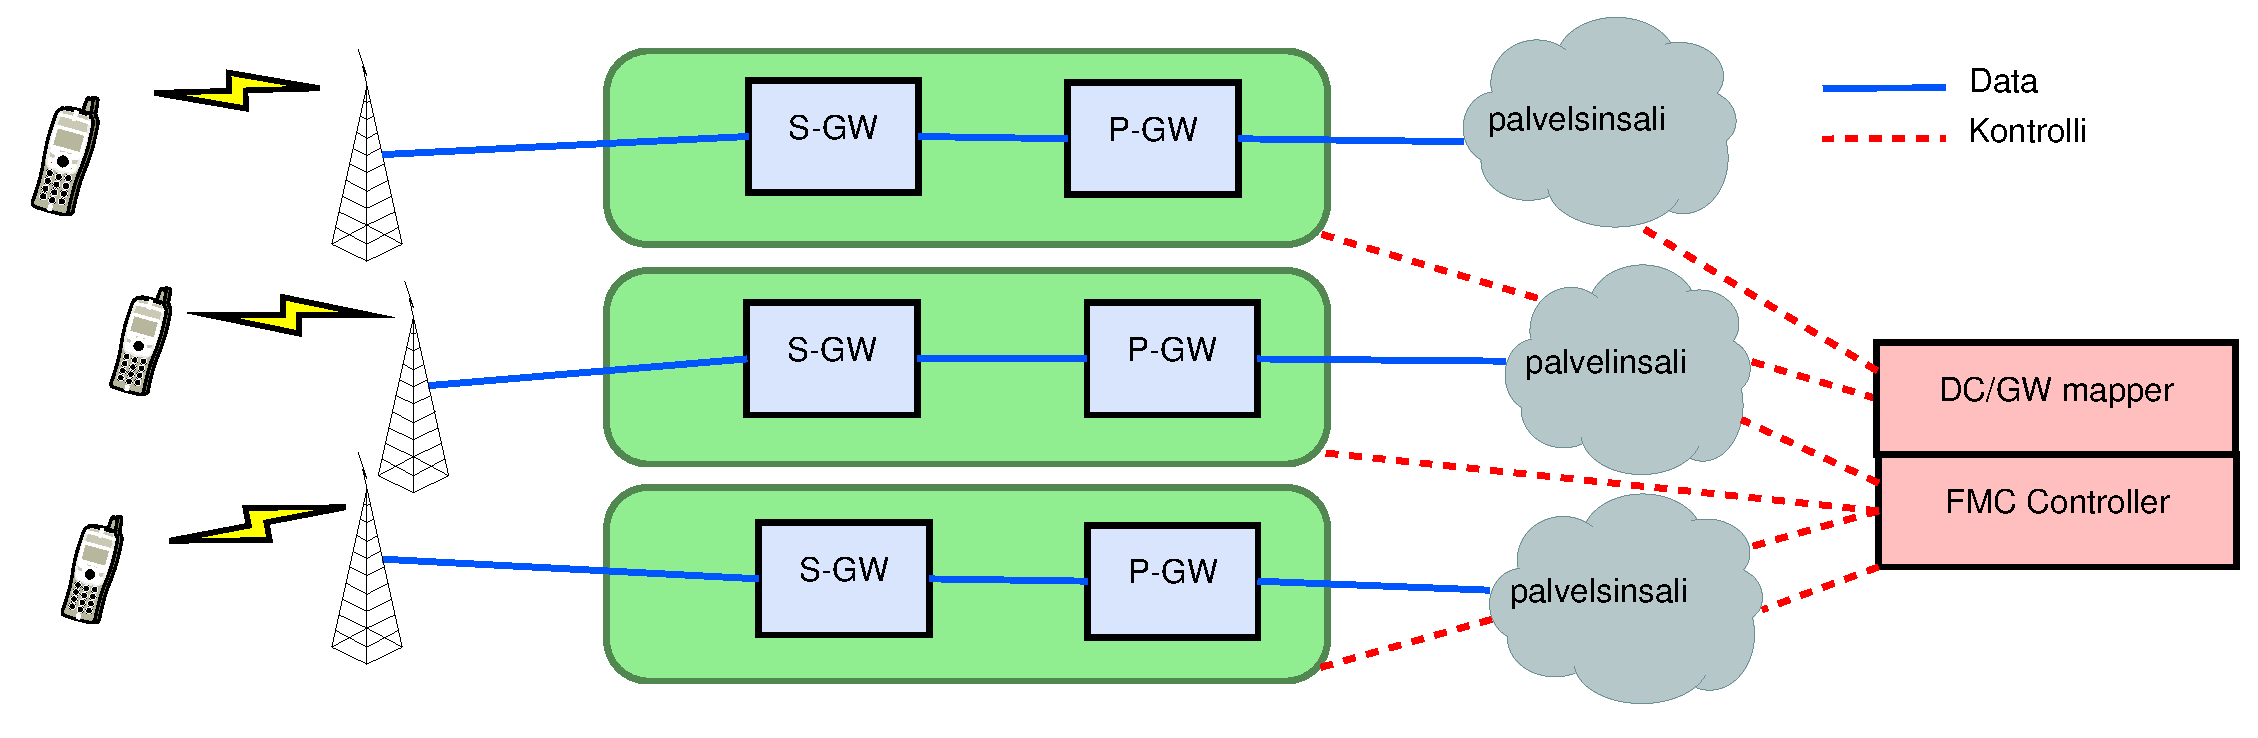
\includegraphics[width = \textwidth]{FMC.eps}
\caption{FMC:n arkkitehtuuri jossa mobiiliverrko on hajautettu} \label{fig:fmc}
\end{figure}

\subsection{FMC - Follow me cloud} \label{fmc}
\paragraph{NOTE} FCM jättää avoimeksi tavan jolla reunan ja reunapalvelun välinen tietoliikenteen ohajus toteutetaan. SDN ottaa tähän enemmän kantaa, mutta sitä ei tässä käsitellä koska se on hyvin samankaltainen kuin MobiScud sekä sijoittuu mobiiliverkon sijaan wlan maailmaan

Asiakaslaitteiden määrän kasvu, sekä tietoliikenne-intensiivisien sovelluksien käytön yleistyminen aiheuttaa suurta kuormaa verkkoinfrastruktuurille. Ongelmat johtuvat pääasiassa keskitetystä rakenteesta, jossa tietoliikenneyhteydet kerätään kulkemaan keskitetyn pisteen kautta. Tämän lisäksi yhteyksissä on huomattavasti viivettä, koska asiakkaan ja palvelimen väliset yhteydet ovat pitkiä. FMC ehdottaa ratkaisua jossa operaattorin keskitetty verkkorakenne muutettaisiin hajautetuksi. \cite{taleb2013follow}
Käytännössä tämä tarkoittaisi, että EPC:n ja ulkoverkon välisten yhdyskäytävien, eli P-GW, määrää lisättäisiin. 
Toinen osa ideaa on, että P-GW:t voitaisiin hajauttaa palvelinsaleihin lähemmäksi asiakkaan käyttämiä palveluita. Tämä siksi, että myös palveluiden tarjoajat ovat huomanneet hajautustarpeen ja alkaneet hajauttaa palveluitaan. 
FMC:n arkkitehtuuri koostuu hajautetusta EPC:stä ja hajautetusta palvelinkeskuksista. Asiakaslaitteen yhdistäessä verkkoon verkkoyhteyksien kiintopisteenä toimii todennäköisimmin lähimpänä sijaitseva P-GW. Perinteisessä mobiiliverkossa asiakaslaite pysyy samana P-GW:n asiakkaana, vaikka liikkuisi mobiiliverkossa. FMC lähteekin ratkaisemaan ongelmaa jossa asiakaslaitteelle tarjottaisiin aina optimaalisin\footnote{optimaalisella tarkoitetaan tässä yhteydessä parasta mahdollista, käyttäen mittareina fyysistä sijaintia ja kuormaa} yhteys tavoiteltuun palveluun.

FMC:n ratkaisemat ongelmat voidaan jakaa kahteen osaa, optimaalisen reitin valitseminen ja optimaalisen reitin ylläpitämiseen käyttäjän liikkuessa. 

Optimaalisella reitinvalinnalla tarkoitetaan, että käyttäjän yhteys kohdepalveluun olisi mahdollisimman lyhyt tai nopea. Tämä jakautuu matkaan, jonka asiakkaan yhteys kulkee mobiiliverkossa, eli tarkemmin ottaen EPC:n sisällä, ja matkaan P-GW:ltä kohdepalvelimeen. Tämän saavuttamiseksi mobiiliverkon arkkitehtuurin tarvitaan palvelinkeskuksien ja P-GW välisiä mappauksia tekevä entiteetti. 

FMC tarjoaa optimaalisen reitin löytämiseen ratkaisua, jossa mobiiliverkkoon lisättäisiin hallitseva entiteetti – FMC Controller. 
Optimaalisen asiakaslaite-palvelinsali -yhteyden ylläpitäminen vaatii jonkin verran muutoksia tapaan jolla käyttäjän siirtymiseen mobiiliverkossa reagoidaan. P-GW:n vaihtaminen ja mahdollisesti myös palvelun tarjoavan konesalin vaihtaminen tarkoittavat että käyttäjän ja palvelun välinen IP-yhteys katkeaa osoitteiden muuttuessa. Kuten kappaleessa \ref{GTP} mainittiin, perinteisessä mobiiliverkko arkkitehtuurissa käyttäjän liikenne ulkoverkkoon kulkee GTP-tunnelia pitkin ja käyttäjän liikkuminen tukiasemien välillä ei näy asiakkaslaitteen yhteyksissä. FMC Controllerin tehtävänä on hoitaa avattujen yhteyksien yhteys-tunnisteita sekä tehdä päätöksiä palveluiden migratoinnista palvelinkeskuksien välillä asiakkaan liikkuessa.

FMC eroaa muista mobiiliverkon ratkaisuista sillä, että se ei tuo palvelinresursseja osaksi mobiiliverkkoa ja pyrkii tekemään mobiili infrastruktuuriin mahdollisimman vähän muutoksia. Sen sijaan FMC pyrkii takaamaan nopeimman mahdollisen yhteyden haluttuun palveluun. FCM jättääkin auki mahdollisuuden, että reunapalvelut tarjoaa joku muu kuin operaattori itse.
